\documentclass[a4paper]{jpconf}
\usepackage{graphicx}
\usepackage{iopams}
\usepackage{hyperref}
\begin{document}
\title{Federating Distributed Storage For Clouds In ATLAS}

\author{Berghaus~F, Casteels~K, Di~Girolamo~A, Driemel~C, Ebert~M, Furano~F, Galindo~F, Lassnig~M, Leavett-Brown~C, Paterson~M, Serfon~C, Seuster~R, Sobie~R, Tafirout~R, Taylor~R~P}

\address{Frank~Berghaus, G07810, CERN, CH-1211 Geneva 23,  Switzerland}

\ead{frank.berghaus@cern.ch}

\begin{abstract}
Input data for applications that run in cloud computing centres can be stored at distant repositories, often with multiple copies of the popular data stored at many sites. Locating and retrieving the remote data can be challenging, and we believe that federating the storage can address this problem. A federation would locate the closest copy of the data on the basis of GeoIP information. Currently we are using the dynamic data federation DynaFed~\cite{dynafed} software solution developed by CERN IT. DynaFed supports several industry standards for connection protocols like Amazon's S3, Microsofts Azure, as well as WebDAV and HTTP. Protocol dependent authentication is hidden from the user by using their X509 certificate. We have setup an instance of DynaFed and integrated it into the ATLAS Data Distribution Management system. We report on the challenges faced during the installation and integration. We have tested ATLAS analysis jobs submitted by the PanDA production system and we report on our first experiences with its operation.
\end{abstract}

\section{Introduction}
Our goal is run data-intensive applications on globally distributed opportunistic resources that have no local grid storage. The ATLAS experiment leverages a globally distributed system of infrastructure as a service clouds, such as Amazon's Web Services, or the Compute Canada, and CERN OpenStack. These resources are integrated into the ATLAS distributed computing system using two cloud scheduler~\cite{cloud-scheduler} instances: one at the University of Victoria and one at CERN. These IaaS resources are used opportunistically, and do not support any local grid infrastructure.

The workflows executed by high energy physics experiments often demand large volumes of input data or produce a significant volume of output data. We aim to use a data federation, such as DynaFed, to redirect the applications running on opportunistic resources to the optimal storage endpoint to retrieve input or deposit output data.

\section{Conceptual Design}
The ATLAS experiment leverages the resources of the Worldwide LHC Computing Grid, WLCG~\cite{wlcg}. The computer centres that are part of the WLCG and support that ATLAS experiment each host some of the experiment data and simulated events. They provide a global storage infrastructure. While the central ATLAS computing infrastructure uses purpose specific protocols to access the content of these grid storage elements, they may be accessed using standard protocols such as WebDAV, HTTP, and NFS. Figure~\ref{fig:conceptual-design} shows how DynaFed could appear to present the entire ATLAS data catalog by unifying the namespaces of attached storage elements.

\begin{figure}
  \centering
  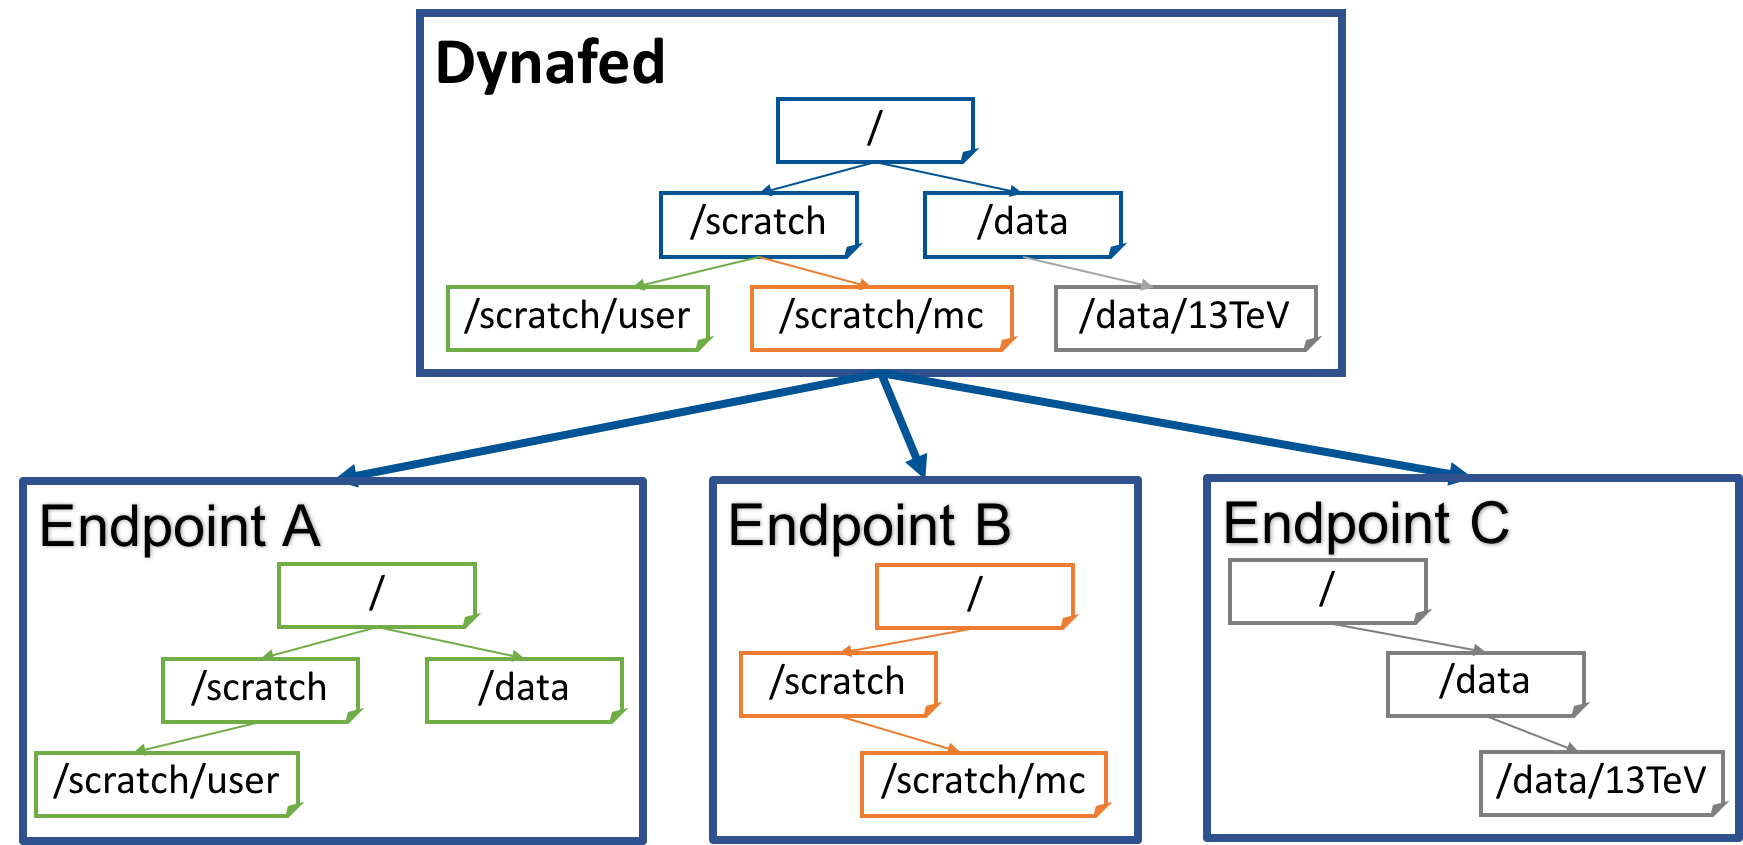
\includegraphics[width=\textwidth]{conceptual-design.png}
  \caption{The dynamic federation is cpnnected to multiple endpoints. Each endpoint may be a file system or an object store accessible using the a protocol which allows redirection. The dynamic federation appears to provide a namespace that is a union of all the namespaces of the endpoints. That namespace is presented as a familiar directory structure on the same protocols as exposed by the endpoints.}
  \label{fig:conceptual-design}
\end{figure}

Cloud storage systems are object stores that expose a well defined interface over HTTP and WebDAV. DynaFed also allows the inclusion of these cloud storage into the a grid system. DynaFed implements authentication through public key infrastructure with grid extensions~\cite{voms} and translates this authentication to authorize access to the cloud storage systems which each have their own authentication and authorization paradigms. Thus a grid user or application authenticates to DynaFed using grid credentials and is forwarded to a pre-signed URL that permits, for a limited time, access to the cloud storage system.

\section{Data Access}


\section{Application Workflow}


\section{Summary}


\section*{Acknowledgments}
Authors wishing to acknowledge assistance or encouragement from
colleagues, special work by technical staff or financial support from
organizations should do so in an unnumbered Acknowledgments section
immediately following the last numbered section of the paper. The
command \verb"\ack" sets the acknowledgments heading as an unnumbered
section.


\section*{References}
\begin{thebibliography}{9}
\bibitem{dynafed}
  Furano~F {\it et al}
  2017
  Dynafed
  \url{http://cern.ch/lcgdm/dynafed-dynamic-federation-project}
\bibitem{cloud-scheduler}
  Gable~I {\it et al}
  2017
  Cloud Scheduler
  \url{http://cloudscheduler.org}
\bibitem{wlcg}
  Bird~I
  2011
  %``Computing for the Large Hadron Collider''
  {\it Ann.\ Rev.\ Nucl.\ Part.\ Sci.\ } {\bf 61} 99
  %doi:10.1146/annurev-nucl-102010-130059
\bibitem{voms}
  Foster~I, Kesselman~C, Tuecke~S
  2001
  %``The Anatomy of the Grid: Enabling Scalable Virtual Organizations''
  {\it International Journal of Supercomputer Applications}
  \url{http://www.globus.org/alliance/publications/papers/anatomy.pdf}


\end{thebibliography}

\end{document}
